% ===================================================================
\section{Calorimetry and the phase-change ledger}\label{sec:calor}
% ===================================================================
\begin{multicols}{2}
\subsection{Heat capacities}\label{sec:heatcap}
\CORE{} \textbf{Cue:} ``specific heat'', ``heat capacity of the cup'', ``water equivalent'', ``J/(mol\,K)''.

\begin{reftab}{T:capacity}{Three bases---keep the basis visible in the units.}
\small
\begin{tabularx}{\linewidth}{@{}lYl@{}}
\toprule
Symbol & Name & Units\\
\midrule
$C$ & total heat capacity of an object & \si{J/K}\\
$c=C/m$ & specific (mass) heat capacity & \si{J/(g.K)}, \si{J/(kg.K)}\\
$\bar c = C/n$ & molar heat capacity & \si{J/(mol.K)}\\
\bottomrule
\end{tabularx}\end{reftab}

\begin{formulabox}
\vspace{-6pt}
\begin{align}
Q &= \int_{T_1}^{T_2} C(T)\,\dd T \;\xrightarrow{\;C\ \text{const}\;}\; Q = mc\,\Delta T \label{F:cal:sensible}\\
c_v &= \Big(\frac{\partial u}{\partial T}\Big)_{\!v},\qquad c_p=\Big(\frac{\partial h}{\partial T}\Big)_{\!p} \label{F:cal:cvcp}
\end{align}
\end{formulabox}
\textbf{Which one?} Closed system, rigid, no work: $Q_V=\Delta U$. Closed system at constant pressure with only boundary work: $Q_P=\Delta H$. Solids and liquids: $c_p\approx c_v$ (tables list $c_p$); gases: $c_p-c_v=R$ per mole (\eqp{F:gas:mayer}).

\textbf{Constant-$c$ shortcut is conditional.} Water's $c_p$ varies only $\pm\SI{0.6}{\percent}$ between 15 and \SI{90}{\celsius} (4.188 to 4.181 to \SI{4.205}{J/(g.K)}),\src{IAPWS} so $c=\SI{4.18}{J/(g.K)}$ is fine; but use the integral (or tabulated $\Delta h$) for wide ranges, for gases over hundreds of kelvin, and near phase changes.

\textbf{Water equivalent} of a container: $m_{\text{eq}}=C_{\text{cal}}/c_{\text{water}}$ (grams of water that would absorb the same energy per kelvin).

\textbf{Dulong--Petit check} (many solid elements near room temperature): $\bar c_p\approx 3R=\SI{24.9}{J/(mol.K)}$, so an unknown metal's molar mass $M\approx 3R/c$. \tref{T:metals} shows 24.2--26.4. Fails for light, stiff solids (diamond, Be, B) and at low $T$.\src{CRC}\src{EK}

\subsection{Water ledger constants}\label{sec:waterconst}
\begin{reftab}{T:waterledger}{Water, ice, steam at \SI{101.325}{kPa} unless stated.\src{IAPWS}\src{ICE}}
\small
\begin{tabularx}{\linewidth}{@{}Yr@{}}
\toprule
Quantity & Value\\
\midrule
$c_p$ liquid, \SI{25}{\celsius} (15 / 90\,\si{\celsius}) & \SI{4.181}{J/(g.K)} (4.188 / 4.205)\\
$c_p$ ice Ih at 0 / $-10$ / \SI{-20}{\celsius} & 2.097 / 2.023 / \SI{1.950}{J/(g.K)}\\
$c_p$ steam: sat.\ vapor / \SI{120}{\celsius} / \SI{150}{\celsius} & 2.080 / 2.021 / \SI{1.986}{J/(g.K)}\\
$L_f$ (fusion) at \SI{0}{\celsius} & \SI{333.4}{J/g} (\SI{6.007}{kJ/mol})\\
$L_v$ at normal boiling point \SI{99.97}{\celsius} & \SI{2256.5}{J/g} (\SI{40.65}{kJ/mol})\\
$L_v$ at \SI{25}{\celsius} (evaporation, at $p_{\text{sat}}$) & \SI{2441.7}{J/g} (\SI{43.99}{kJ/mol})\\
$L_{\text{sub}}$ near triple point $\approx L_f+L_v(\SI{0.01}{\celsius})$ & $\approx\SI{2834}{J/g}$\\
$\rho$ liquid \SI{25}{\celsius} / ice \SI{0}{\celsius} & 997.0 / \SI{916.7}{kg/m^3}\\
\bottomrule
\end{tabularx}\end{reftab}
Textbook roundings $c=4.18$ or 4.184, $L_f=334$, $L_v=2260$ are acceptable \emph{if a question states them}; use the given values when supplied.

\subsection{The energy ledger}\label{sec:ledger}
\CORE{} \textbf{Cue:} ``mixed'', ``dropped into'', ``final temperature'', ``unknown metal'', ``heater''.
\begin{formulabox}For bodies $i$ inside an insulated, constant-pressure enclosure, with net energy input $E_{\text{in}}$ (electrical, stirring) and leak $Q_{\text{loss}}$:
\begin{equation}
\sum_i \Delta H_i \;=\; E_{\text{in}} - Q_{\text{loss}}, \label{F:cal:ledger}
\end{equation}
each $\Delta H_i$ a sum of sensible pieces $m_ic_i(T_f-T_{i})$ and latent pieces $\pm m L$ ($+$ for melting/boiling, $-$ for freezing/condensing).
\end{formulabox}
\textbf{No phase change, no input, no leak, constant $C$:}
\begin{equation}
T_f=\frac{\sum_i C_iT_i}{\sum_i C_i},\qquad C_i=m_ic_i. \label{F:cal:mixT}
\end{equation}

\begin{keybox}\textbf{Ledger algorithm.} (1) List \emph{every} body: samples, water, cup, stirrer, probe. (2) Hypothesize the final state (temperature region and phases). (3) Write each $\Delta H_i$ with signed $(T_f-T_i)$---no ``lost/gained'' bookkeeping. (4) Sum to $E_{\text{in}}-Q_{\text{loss}}$ and solve. (5) Reject and redo if the result contradicts the hypothesis (e.g.\ $T_f>\SI{0}{\celsius}$ while ice remains, or melted mass $<0$ or $>$ available).\end{keybox}

\begin{trapbox}With no external input, $T_f$ must lie between the lowest and highest initial temperatures. A result outside that range signals a sign error, a missed phase change, an unaccounted reaction or electrical input, or a wrong capacity. ``Heat lost = heat gained'' with magnitudes invites sign errors; the signed sum cannot.\end{trapbox}

\subsection{Phase-change decision procedure}\label{sec:phasedecision}
\CORE{} Ice (at $T_{\text{ice}}\le0$) added to warm water (plus cup) at $T_w$; at 1~atm use $\SI{0}{\celsius}$ as the melting point. Define the energy terms with all capacities $>0$:
\begin{align*}
Q_{\text{av}} &= (m_wc_w + C_{\text{cup}})\,(T_w-0) && \text{warm side}\to\SI{0}{\celsius}\\
Q_{1} &= m_ic_{\text{ice}}\,(0-T_{\text{ice}}) && \text{ice}\to\SI{0}{\celsius}\\
Q_{2} &= m_iL_f && \text{melt all ice}
\end{align*}
\begin{keybox}\textbf{Decide by comparing energies, never by guessing $T_f$:}
\begin{enumerate}
\item $Q_{\text{av}}<Q_1$: some \emph{water freezes}; frozen mass $=(Q_1-Q_{\text{av}})/L_f$. If that exceeds $m_w$, everything freezes and $T_f<\SI{0}{\celsius}$ (solve sensible ledger).
\item $Q_1\le Q_{\text{av}}<Q_1+Q_2$: $T_f=\SI{0}{\celsius}$; melted mass $=(Q_{\text{av}}-Q_1)/L_f$.
\item $Q_{\text{av}}\ge Q_1+Q_2$: all melts; $T_f=\dfrac{Q_{\text{av}}-Q_1-Q_2}{(m_w+m_i)c_w+C_{\text{cup}}}$.
\end{enumerate}
Steam (at $T_{\text{sat}}$) into cool water: same logic at $T_{\text{sat}}(P)$ (\tref{T:water:satP}), with condensation energy $m_sL_v$ released first.\end{keybox}

\begin{demobox}\textbf{Partial melt.} \SI{100.0}{g} ice at \SI{-10.0}{\celsius} into \SI{200.0}{g} water at \SI{25.0}{\celsius} in a cup with $C_{\text{cup}}=\SI{10}{J/K}$; $c_w=4.18$, $c_{\text{ice}}=\SI{2.03}{J/(g.K)}$, $L_f=\SI{333.4}{J/g}$.
$Q_{\text{av}}=(836+10)(25)=\SI{21150}{J}$; $Q_1=100(2.03)(10)=\SI{2030}{J}$; $Q_2=\SI{33340}{J}$.
Case 2 applies ($2030\le21150<35370$): $T_f=\SI{0}{\celsius}$, melted $=(21150-2030)/333.4=\SI{57.35}{g}$, so \SI{42.65}{g} of ice remains.
\emph{Check:} signed ledger $-21150+2030+57.35(333.4)=0$ \checkmark; $0<57.35<100$ \checkmark.\end{demobox}

\begin{demobox}\textbf{Steam condenses.} \SI{10.0}{g} steam at \SI{100}{\celsius} into \SI{200.0}{g} water at \SI{20.0}{\celsius} (ignore cup; $L_v=\SI{2256.5}{J/g}$, $c_w=4.18$): $10(-2256.5)+10(4.18)(T_f-100)+200(4.18)(T_f-20)=0\Rightarrow T_f=\SI{49.5}{\celsius}$. Only \SI{10}{g} of steam raises \SI{200}{g} of water by \SI{29.5}{K}: latent energy dominates.\end{demobox}

\subsection{Heating curve}\label{sec:heatingcurve}
\begin{reffig}{fig:heatingcurve}{Heating curve of \SI{1.00}{kg} \ce{H2O} at \SI{101.325}{kPa}, drawn to scale from IAPWS enthalpy differences.\src{IAPWS}\src{ICE} Plateaus: constant $T$ while phase changes. Sloped segments: slope $=1/(mc_p)$, so ice and steam rise about twice as steeply as liquid water.}
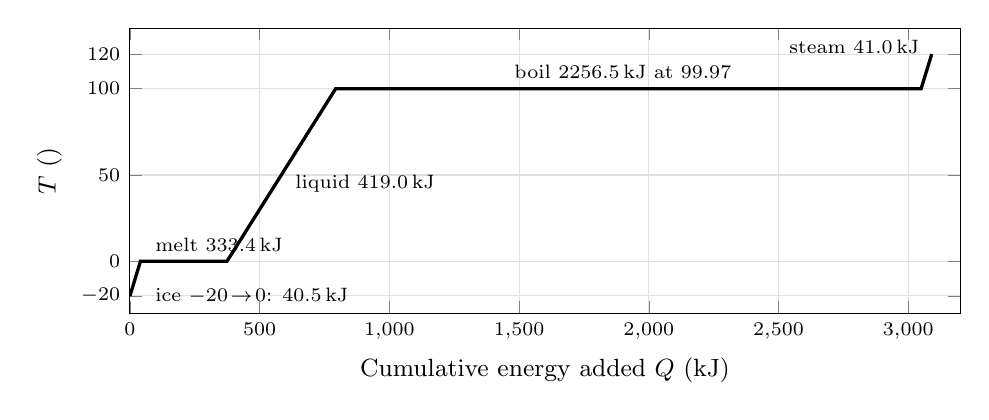
\begin{tikzpicture}
\begin{axis}[width=\linewidth,height=5.2cm,xmin=0,xmax=3200,ymin=-30,ymax=135,
  xlabel={Cumulative energy added $Q$ (\si{kJ})},ylabel={$T$ (\si{\celsius})},
  ytick={-20,0,50,100,120},xtick={0,500,1000,1500,2000,2500,3000},
  tick label style={font=\scriptsize},label style={font=\small},
  grid=major,grid style={black!12},scaled x ticks=false]
\addplot[very thick,black] coordinates {(0,-20)(40.5,0)(373.9,0)(792.9,99.97)(3049.4,99.97)(3090.4,120)};
\node[font=\scriptsize,anchor=south west] at (axis cs:60,0) {melt 333.4\,kJ};
\node[font=\scriptsize,anchor=south] at (axis cs:1900,100) {boil 2256.5\,kJ at \SI{99.97}{\celsius}};
\node[font=\scriptsize,anchor=west] at (axis cs:600,45) {liquid 419.0\,kJ};
\node[font=\scriptsize,anchor=west] at (axis cs:60,-20) {ice $-20\!\to\!0$: 40.5\,kJ};
\node[font=\scriptsize,anchor=east] at (axis cs:3080,124) {steam 41.0\,kJ};
\end{axis}
\end{tikzpicture}
\end{reffig}

\subsection{Calorimeters and corrections}\label{sec:calorimeters}
\CORE{}
\begin{formulabox}
\vspace{-6pt}
\begin{align}
&\text{Coffee cup (constant }P\text{), }\Delta H\approx q_{\text{rxn}}:\notag\\
&\qquad q_{\text{rxn}}=-(m_{\text{soln}}c_{\text{soln}}+C_{\text{cal}})\,\Delta T \label{F:cal:cup}\\
&\text{Bomb (constant }V\text{), }\Delta U\approx q_{\text{rxn}}:\notag\\
&\qquad q_{\text{rxn}}=-C_{\text{bomb}}\,\Delta T \label{F:cal:bomb}\\
&\text{Electrical: }E_{\text{in}}=VIt=I^2Rt=\tfrac{V^2}{R}\,t \label{F:cal:elec}
\end{align}
\end{formulabox}
Divide $q_{\text{rxn}}$ by moles of the \emph{limiting} reactant for a molar $\Delta H$; then convert bomb $\Delta U$ to $\Delta H$ with \eqp{F:thermo:bomb}.

\textbf{Coffee-cup assumptions:} negligible exchange with the room during the run (foam cup, lid), solution $c$ and density $\approx$ water's (often $\SI{4.18}{J/(g.K)}$, \SI{1.00}{g/mL}), complete reaction, no gas or vapor loss. \textbf{Bomb:} calibrated $C_{\text{bomb}}$ from a standard (benzoic acid); corrections for ignition-wire energy, acid formation, and jacket exchange.\src{EK} Neither is lossless.

\textbf{Heater energy $\ne$ sample energy.} $E_{\text{in}}$ is split among sample, container, heater, probe, and losses. Electrical calibration: $C_{\text{total}}=E_{\text{in}}/\Delta T$ for the whole assembly.

\textbf{Heat-leak (drift) correction.} Record $T$ before and after mixing; extrapolate both linear (or exponential) drift lines to the moment of mixing and take $\Delta T$ between the extrapolations. This approximately removes exchange with the room during slow mixing.\src{EK}

\begin{reffig}{fig:drift}{Heat-leak (drift) correction, schematic (axes not to scale). Extrapolate the pre- and post-event drift lines to the mixing time $t_{\text{mix}}$; use $\Delta T$ between them, not the raw peak.\src{EK}}
\begin{tikzpicture}[font=\scriptsize,>=Stealth]
 \draw[->] (0,0)--(6.6,0) node[below left]{$t$};
 \draw[->] (0,0)--(0,3.1) node[above right]{$T$};
 \draw[thick] (0.2,0.75)--(2.2,0.85);
 \draw[thick] (2.2,0.85) .. controls (2.5,2.3) and (2.9,2.55) .. (3.4,2.55);
 \draw[thick] (3.4,2.55)--(6.3,2.25);
 \draw[dashed] (2.2,0.85)--(2.6,0.87);
 \draw[dashed] (3.4,2.55)--(2.4,2.65);
 \draw[densely dotted] (2.4,0)--(2.4,2.9) node[above]{$t_{\text{mix}}$};
 \draw[<->] (2.75,0.86)--(2.75,2.63) node[midway,right]{$\Delta T_{\text{corr}}$};
 \node[anchor=west] at (3.9,2.65){slow cooling (leak)};
 \node[anchor=west] at (0.2,0.5){baseline drift};
\end{tikzpicture}
\end{reffig}

\begin{demobox}\textbf{Electrical calibration.} A heater at \SI{12.0}{V}, \SI{1.50}{A} for \SI{300}{s} delivers $E=\SI{5400}{J}$ to a cup holding \SI{250}{g} water; drift-corrected $\Delta T=\SI{4.95}{K}$. $C_{\text{total}}=5400/4.95=\SI{1091}{J/K}$; minus water ($250\times4.18=\SI{1045}{J/K}$) gives $C_{\text{cal}}\approx\SI{46}{J/K}$. Small differences of large numbers: a \SI{0.05}{K} error in $\Delta T$ shifts $C_{\text{cal}}$ by about \SI{11}{J/K}.\src{DER}\end{demobox}

\begin{demobox}\textbf{Calorimeter constant.} \SI{50.0}{g} water at \SI{60.0}{\celsius} poured into a cup holding \SI{50.0}{g} water at \SI{20.0}{\celsius}; $T_f=\SI{38.6}{\celsius}$; $c=\SI{4.184}{J/(g.K)}$.
Hot water: $50(4.184)(38.6-60.0)=\SI{-4477}{J}$. Cold water: $50(4.184)(18.6)=\SI{+3891}{J}$. Cup: $+\SI{586}{J}$ over \SI{18.6}{K} $\Rightarrow C_{\text{cal}}=\SI{31.5}{J/K}$ (water equivalent \SI{7.5}{g}).
\emph{Check:} re-solving \eqref{F:cal:ledger} with $C_{\text{cal}}=31.49$ returns $T_f=\SI{38.60}{\celsius}$ \checkmark.\end{demobox}

\begin{demobox}\textbf{Unknown metal, and why the cup matters.} \SI{100.0}{g} metal at \SI{98.0}{\celsius} into \SI{150.0}{g} water at \SI{22.0}{\celsius} in that cup ($C_{\text{cal}}=\SI{31.5}{J/K}$); $T_f=\SI{26.2}{\celsius}$.
$c_m=\dfrac{(150\cdot4.184+31.5)(4.2)}{100\,(71.8)}=\SI{0.386}{J/(g.K)}$. Ignoring the cup gives 0.367 (\SI{5}{\percent} low).
\emph{Resolution:} $\pm\SI{0.1}{K}$ on $T_f$ gives 0.376--0.395, which contains Cu (0.384) \emph{and} Zn (0.388) but excludes Fe, Al, Ni (\tref{T:metals}). Dulong--Petit: $M\approx24.9/0.386=\SI{65}{g/mol}$---still Cu or Zn. A second property (density) is needed. Report the range, not a false identification.\end{demobox}

\begin{trapbox}Common ledger errors: forgetting the cup/probe; using \SI{100}{\celsius} for boiling at altitude; using $L_v$ at \SI{100}{\celsius} for room-temperature evaporation (\SI{2441.7}{J/g} at \SI{25}{\celsius}); using $c_{\text{water}}$ for ice or steam; mixing grams with kilograms or J with cal ($1\,\mathrm{cal_{th}}=\SI{4.184}{J}$; food Calorie $=1$~kcal); using a molar $\bar c$ with a mass.\end{trapbox}
\end{multicols}
